
Commençons par introduire les données fonctionnelles de manière informelle afin de mieux intégrer la définition formelle, plus utile pour la manipulation.

Cette section regroupe l'ensemble des messages essentiels à retenir des données fonctionnelles pour la pratique, sans alourdir les notions avec des notations mathématiques. Le cadre formel sera traité juste après.

\begin{definition*}[données fonctionnelles — informel]
    Les données fonctionnelles sont des données dont les observations sont des fonctions, c'est-à-dire des courbes, des surfaces, des images, \, \dots
    
    i.e : toute donnée ayant une dépendance de type "relation fonctionnelle" avec un ou plusieurs paramètres.
    \label{def*:fda}
\end{definition*}

\begin{figure}[H]
    \begin{center}
        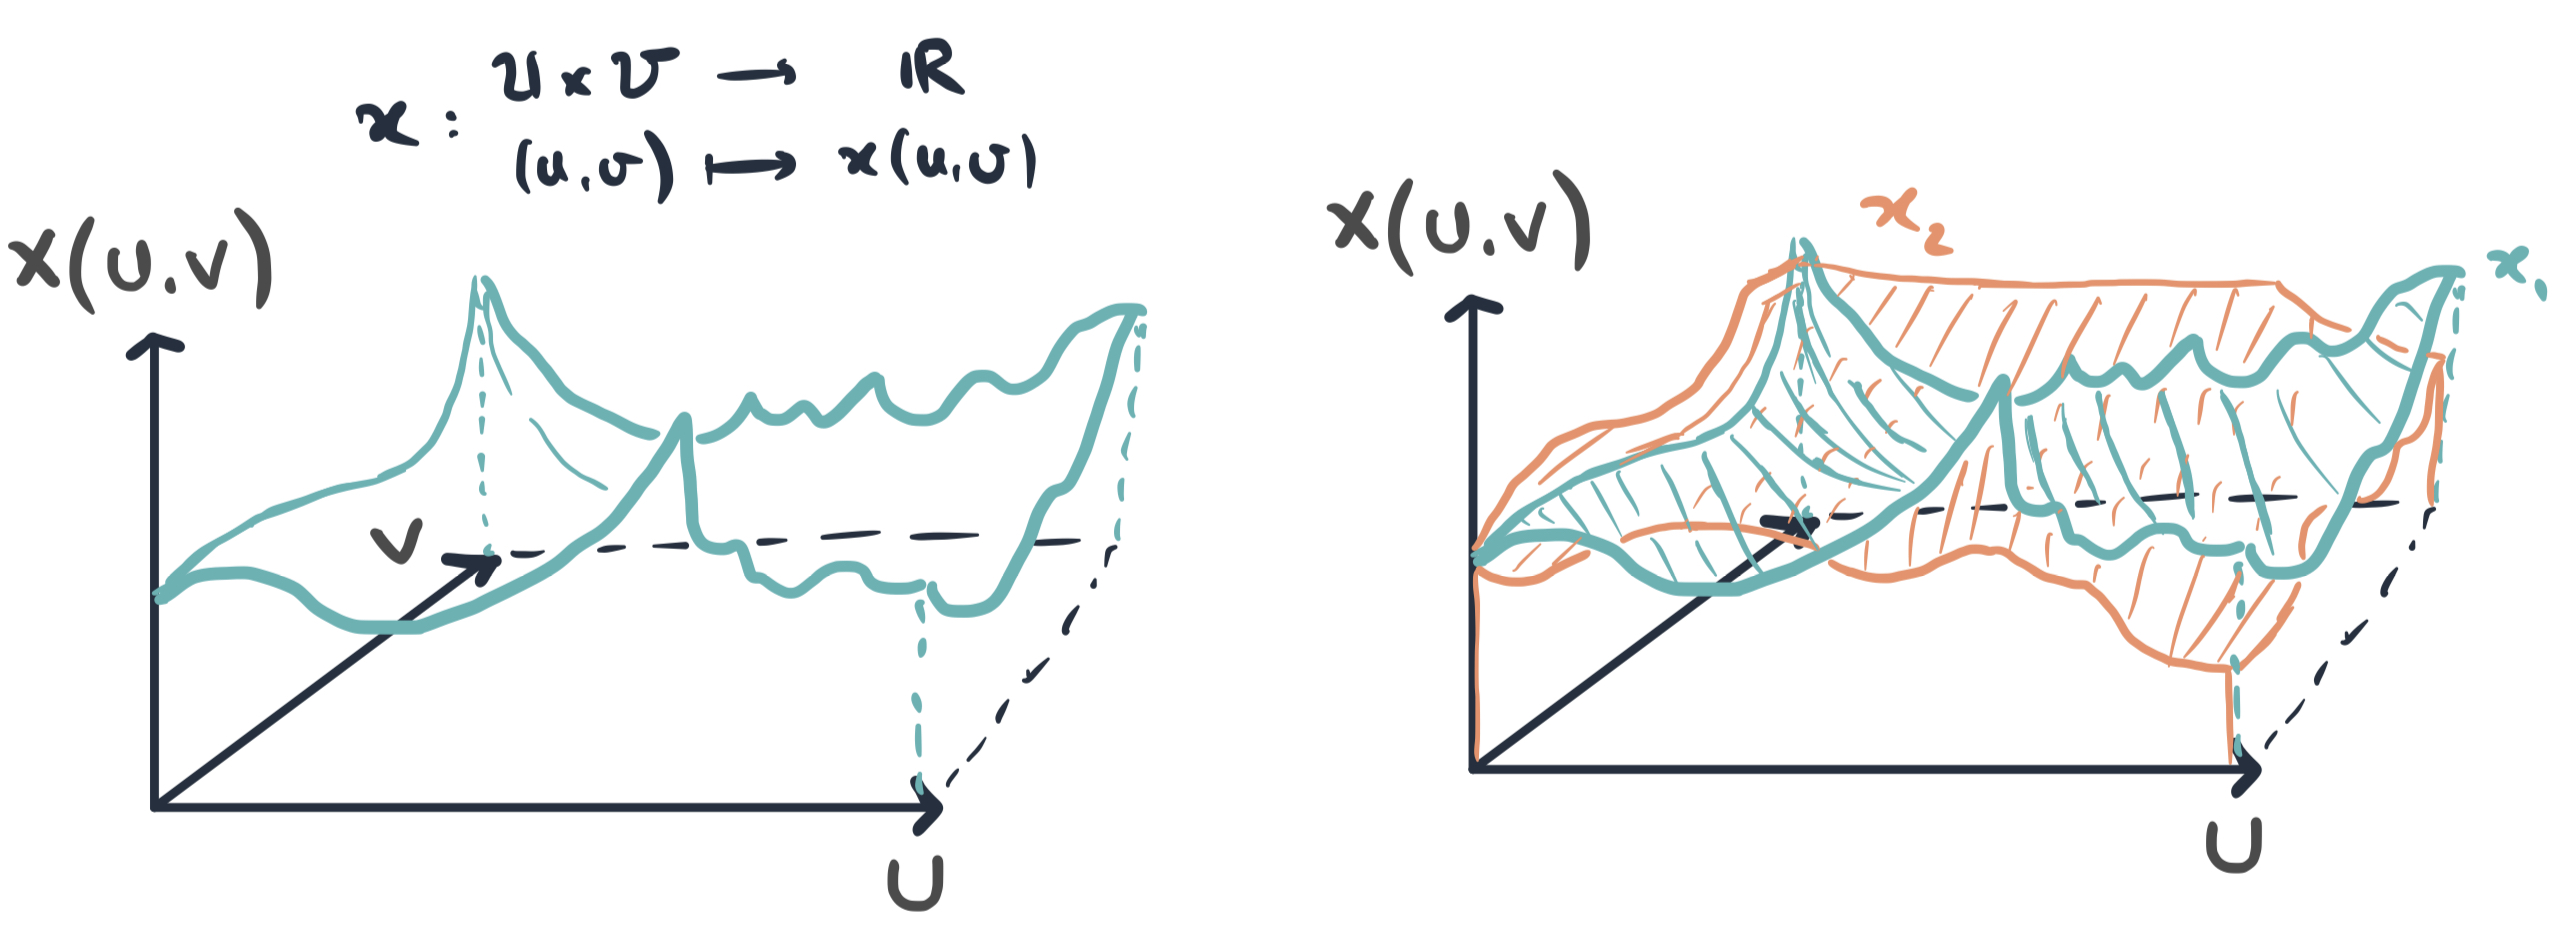
\includegraphics[width=\textwidth]{Images/sketches/fda_surface.jpg}
    \end{center}
    
    {
    \textbf{Gauche :} exemple de surface
    \\
    \textbf{Droite :} échantillon de deux observations de la surface suivant une loi fonctionnelle}

    \caption{Donnée fonctionnelle : relation fonctionnelle avec plusieurs paramètres}
    \label{fig:sketch_surface}
\end{figure}

Maintenant introduites, les théorèmes suivant permettent de manipuler ces données à la fois pour la théorie et la pratique :

\begin{thm*}[\nameref{thm:KL} — informel]
    \noindent\fbox{%
    \parbox{\textwidth}{%
    Il est possible pour une large classe de données fonctionnelles de les décomposer dans une base \emph{de fonctions} adaptée aux données (au sens de la covariance) que l'on appelle base ACP fonctionelle (FPCA).
    }%
    }
    \label{thm*:KL}
\end{thm*}
\begin{proof}[\faCogs \, preuve informelle]
    La covariance est un opérateur bilinéaire symétrique défini positif, on peut donc appliquer le théorème de Mercer (équivalent du théorème spectral) qui nous donne une base orthonormale de $\mathds L^2$ sur laquelle on va décomposer notre processus \textbf{centré}.
\end{proof}
\begin{rem}
    La classe de fonctions pouvant être décomposées est large, puisqu'elle regroupe l'ensemble des processus qui nous intéressent la plus part du temps en tant que statisticien : celles qui sont à support sur un intervalle, admettant une covariance continue et finie sur le support.
\end{rem}
    
On en déduit que pour travailler avec des données fonctionnelles, il suffit de les décomposer dans la base ACP fonctionnelle puis de travailler sur les composantes de chaque élément de la base. On travaille désormais avec des réels et non plus des fonctions, ce qu'on aime manipuler. On peut alors faire de la statistique traditionnelle avec les outils que l'on connait.


\begin{propriete*}[intérêt de la base FPCA — informel]
    \noindent\fbox{%
    \parbox{\textwidth}{%
    la base ACP fonctionnelle est la plus économe, c'est à dire qu'elle explique au mieux la covariance des données pour un nombre de composantes fixées, ce qui est utile car on ne sait manipuler numériquement que des objets de dimension finie.
    }%
    }
\end{propriete*}

\subsection{estimation adaptative informelle}

On a mentionné qu'il serait judicieux de lisser les observations en tenant compte de la régularité du processus dont est issu nos données. La question est désormais la suivante :

\question{
    Est-il possible de récupérer la régularité locale des trajectoires à partir des données ? Si oui, comment ?
}

C'est ce qu'affirme le théorème suivant à partir des travaux de Golovkine et al. ainsi que Maissoro-Patilea-Vimond (MPV) :

\begin{thm*}[Regularité locale — informel]
    \noindent\fbox{%
    \parbox{\textwidth}{%
    Les données fonctionnelles permettent de récupérer la régularité locale des trajectoires. Les estimateurs définis \textbf{ponctuellement} convergent. 
    }%
    }
    \label{thm*:regularite_locale}
\end{thm*}
\begin{rem}[Continuité de Kolmogorov]
    Un théorème (\nameref{thm:kolmogorov_continuite}) permet à partir de l'espérance d'incréments d'un processus aléatoire de déduire sa régularité.
    C'est pourquoi les estimateurs sont définis à partir de l'espérance des incréments quadratiques du processus. C'est entre autres \emph{la raison pour laquelle les données fonctionnelles permettent de récupérer la régularité locale des trajectoires}.

    \label{rem:kolmo_continuite}
\end{rem}

Les motivations de l'obtention de la régularité étaient en partie de pouvoir mieux estimer les quantités qui nous intéressent dont la fonction moyenne du processus, ainsi que son opérateur de covariance. Ce qui est à la fois important pour l'analyse (via l'interprétation de la base ACP déterminée par la covariance) et pour la prédiction. On peut alors se demander si il existe des estimateurs de la moyenne et de la covariance prenant en compte la régularité locale. C'est ce qu'affirme les théorèmes suivants :

\warn{demander à Hassan la dernière version de son papier car la partie d estimation adaptative a beaucoup changé}

\begin{thm*}[Estimateurs de la moyenne et de la covariance — informel ~\cite{golovkine2021adaptive}]
    \noindent\fbox{%
    \parbox{\textwidth}{%
    Il est possible en lissant les observations par méthode à noyaux avec une largeur de bande \emph{spécifique à l'objet que l'on souhaite estimer}, de dériver des estimateurs de la moyenne et de la covariance qui convergent. 
    La largeur de bande optimale \emph{pour l'objet que l'on souhaite estimer} est celle qui minimise un risque qui effectue un compromis biais-variance, qui dépend de la régularité locale du processus, en pénalisant les largeurs de bande menant à des "trous" dans les fonctions lissées.
    On parle d'\emph{\og estimation adaptative \fg}.
    }%
    }

    \label{thm*:estimation_adaptative}
\end{thm*}

Cependant, bien qu'une largeur de bande optimale existe, elle est inconnue. Il est donc important de savoir si le praticien peut l'estimer, et avec quelle précision (c'est à dire à quel point l'estimateur sera biaisé ou non). C'est ce que nous affirme le théorème suivant :

\pagebreak

\begin{thm*}[expression de la largeur de bande optimale — informel ~\cite{golovkine2021adaptive}]
    \noindent\fbox{%
    \parbox{\textwidth}{%
    Sous certaines hypothèses de régularité du processus, et d'indépendance des temps observés, la largeur de bande optimale peut être approchée (avec forte probabilité de bonne approximation) par une expression ne dépendant que du nombre de courbes observées, du nombre moyen de temps observés par courbe, et de la régularité locale du processus. Ce biais de l'estimateur de la fonction moyenne est alors contrôlé en fonction de ces mêmes quantités.

    Sous des hypothèses un peu plus fortes sur le nombre d'observations par courbe, et le nombre de courbe on dispose de résultats similaires pour l'estimateur de la covariance.}%
    }
        
    \label{thm*:h_opt_estim}
\end{thm*}


Enfin, on peut se demander ce qu'il en est des estimateurs dans le cadre où l'on dispose de la dépendance dans les données (ce qui est la cas pour les données éoliennes notamment). Ce cas est traîté par le théorème suivant dérivé par MPV :

\begin{thm*}[ Estimation adaptative de séries temporelles fonctionnelles — informel ~\cite{maissoro-SmoothnessFTSweakDep} ]

    On peut estimer la régularité d'une série temporelle de données fonctionnelles à condition que la mémoire temporelle de la série soit courte. (La décroissance de la dépendance temporelle doit être au moins aussi rapide qu'une décroissance géométrique)

    \label{thm*:far_adaptative_estimation}
\end{thm*}

\pagebreak

\subsection{Résumé informel de la méthodologie}

Les données fonctionnelles permettent de travailler sur un modèle où la \emph{relation} entre plusieurs quantités est sujet à une loi \colorize[flatuicolors_biscay]{[$cf$ \nameref{def*:fda}]}. Ce point de vue de réplication de courbes est notamment utile car il permet d'extraire des observations leur régularité \colorize[flatuicolors_biscay]{[$cf$ \nameref{rem:kolmo_continuite}, \nameref{thm*:regularite_locale}]}. L'estimation de cette régularité permet, entre autres, de lisser les courbes de façon appropriée en fonction de la quantité que l'on souhaite estimer, telle que la moyenne et la covariance avec une plus grande précision \colorize[flatuicolors_biscay]{[$cf$ \nameref{thm*:estimation_adaptative}]}. 

\noindent\begin{figure}[H]
    \centering
    \pagewidthimg{Images/sketches/sketch_resume_informel.jpg}
    \caption{Résumé des motivations du de l'estimation de la régularité locale des trajectoires}
    \label{fig:sketch_resume_informel}
\end{figure}


\pagebreak